\documentclass[10pt,t]{beamer}

\usepackage[utf8]{inputenc}
\usepackage[T1]{fontenc}
\usepackage{graphicx}
\usepackage{grffile}
\usepackage{longtable}
\usepackage{wrapfig}
\usepackage{rotating}
\usepackage[normalem]{ulem}
\usepackage{amsmath}
\usepackage{textcomp}
\usepackage{amssymb}
\usepackage{capt-of}
\usepackage{hyperref}

\input beamer_setup

\usetheme{default}
% ---------------------------------------------------------------------
% ---------------------------------------------------------------------
\title[Retrievals]{Progress on the AIRS RTA}
\author{Sergio DeSouza-Machado, Larrabee
  Strow, Chris Hepplewhite} \institute{Department of Physics, JCET\\
  University of Maryland Baltimore County (UMBC)} \date{October 4, 2018}
% ---------------------------------------------------------------------
% ---------------------------------------------------------------------
\begin{document}
% ---------------------------------------------------------------------
% ---------------------------------------------------------------------
\begin{frame}
  \titlepage
\end{frame}
% ---------------------------------------------------------------------
\begin{frame}
  \frametitle{Overview}

  \begin{itemize}
  \item Generally spectroscopy is the main contributor to RTA error
  \item UMBC is unique in that we can mix/match UMBC-LBL with LBLRTM
  \item Some real advancements in lineshapes now taking place, compared to
    last 10 years
  \item We are working to get these into SARTA quickly, are interacting
    with HITRAN (Harvard-Smithsonian), AER (LBLRTM), and CNRS (Hartmann) to
    ingest latest algorithms.
  \item More SARTA parametrization work necessary:
    \begin{itemize}
    \item Improve fitting (neural net, etc), using thousands of training
      profiles
    \item Can now provide error covariance matrix for SARTA
      parametrization errors
    \item \emph{Want to greatly simplify fitting code and SARTA for ease of
        use by others in the future}.  This is a big job, but we want to get
      there.
    \end{itemize}
  \end{itemize}

\end{frame}
% ---------------------------------------------------------------------
\begin{frame}[shrink=5]
  \frametitle{RTA development at UMBC}
  \vspace{0.125in} 
  \begin{description}
  \item[kCARTA:]

    \textit{kCompressed Atmospheric Radiative Transfer Algorithm}\\
    \begin{itemize}
    \item Two versions: Matlab, f90
    \item Based on $\sim$1 Gbyte compressed look-up tables
    \item 45 seconds for full radiance spectrum
    \item 0.0025 \wn spectral resolution, averaged from 0.0005 \wn data
      grid
    \end{itemize}

  \item [SARTA:] \emph{Stand Alone Rapid Transmittance Algorithm }\\
    \begin{itemize}
    \item Used by NOAA NUCAPS and NASA EOS-AIRS
    \item Regressions over kCARTA generated optical depths
    \item 0.03 seconds for 2255 channels
    \item Training sets: UMBC profiles (49), TIGR (about 2000), ECMWF
      (25000)
    \end{itemize}
    \textcolor{maroon}{SARTA Scattering: TwoSlab cloud representation for
      single footprint retrievals and for validation under partly cloudy
      scenes.}
  \end{description}
\end{frame}
% ---------------------------------------------------------------------
\begin{frame}
  \frametitle{Code Base}
  \vspace{-0.1 in}
  \begin{description}
  \item [UMBC Line-by-Line RTA:] Voigt-VanHuber lineshape, cross-section
    gases, UMBC CO2 line mixing, Hartman line mixing; switches for HITRAN 1996-2016, GEISA 2015,MT-CKD continuum, ...
  \item [AER LBLRTM:] Latest versions (12.4,12.8) have \cd/\methane
    line mixing, plus MT-CKD continuum
  \item[kCARTA:] Built (look-up tables) from \emph{both} LBL's listed
    above!  kCARTA allows us to use 100's to 1000's of fitting profiles
    Includes scattering if desired.
  \item[SARTA:] Fast RTA model using in NUCAPS.  Built from kCARTA.
    Includes 2-slab cirrus/water/aerosol scattering. (Cris NSR, CrIS FSR,
    AIRS, IASI)
  \end{description}

  \vspace{-0.0625in} \textbf{Single Footprint Retrievals : stay tuned till this afternoon}
  \vspace{-0.0625in}
  \begin{itemize}
  \item Used to test SARTA performance
  \item Allows radiosonde inter-comparisons under some cloud cover
  \item Examine single footprint fitting residuals to uncover issues
  \end{itemize}

\end{frame}
% ---------------------------------------------------------------------
% \begin{frame}
%   \frametitle{Flow Diagram}
%   \begin{center}
%     \noindent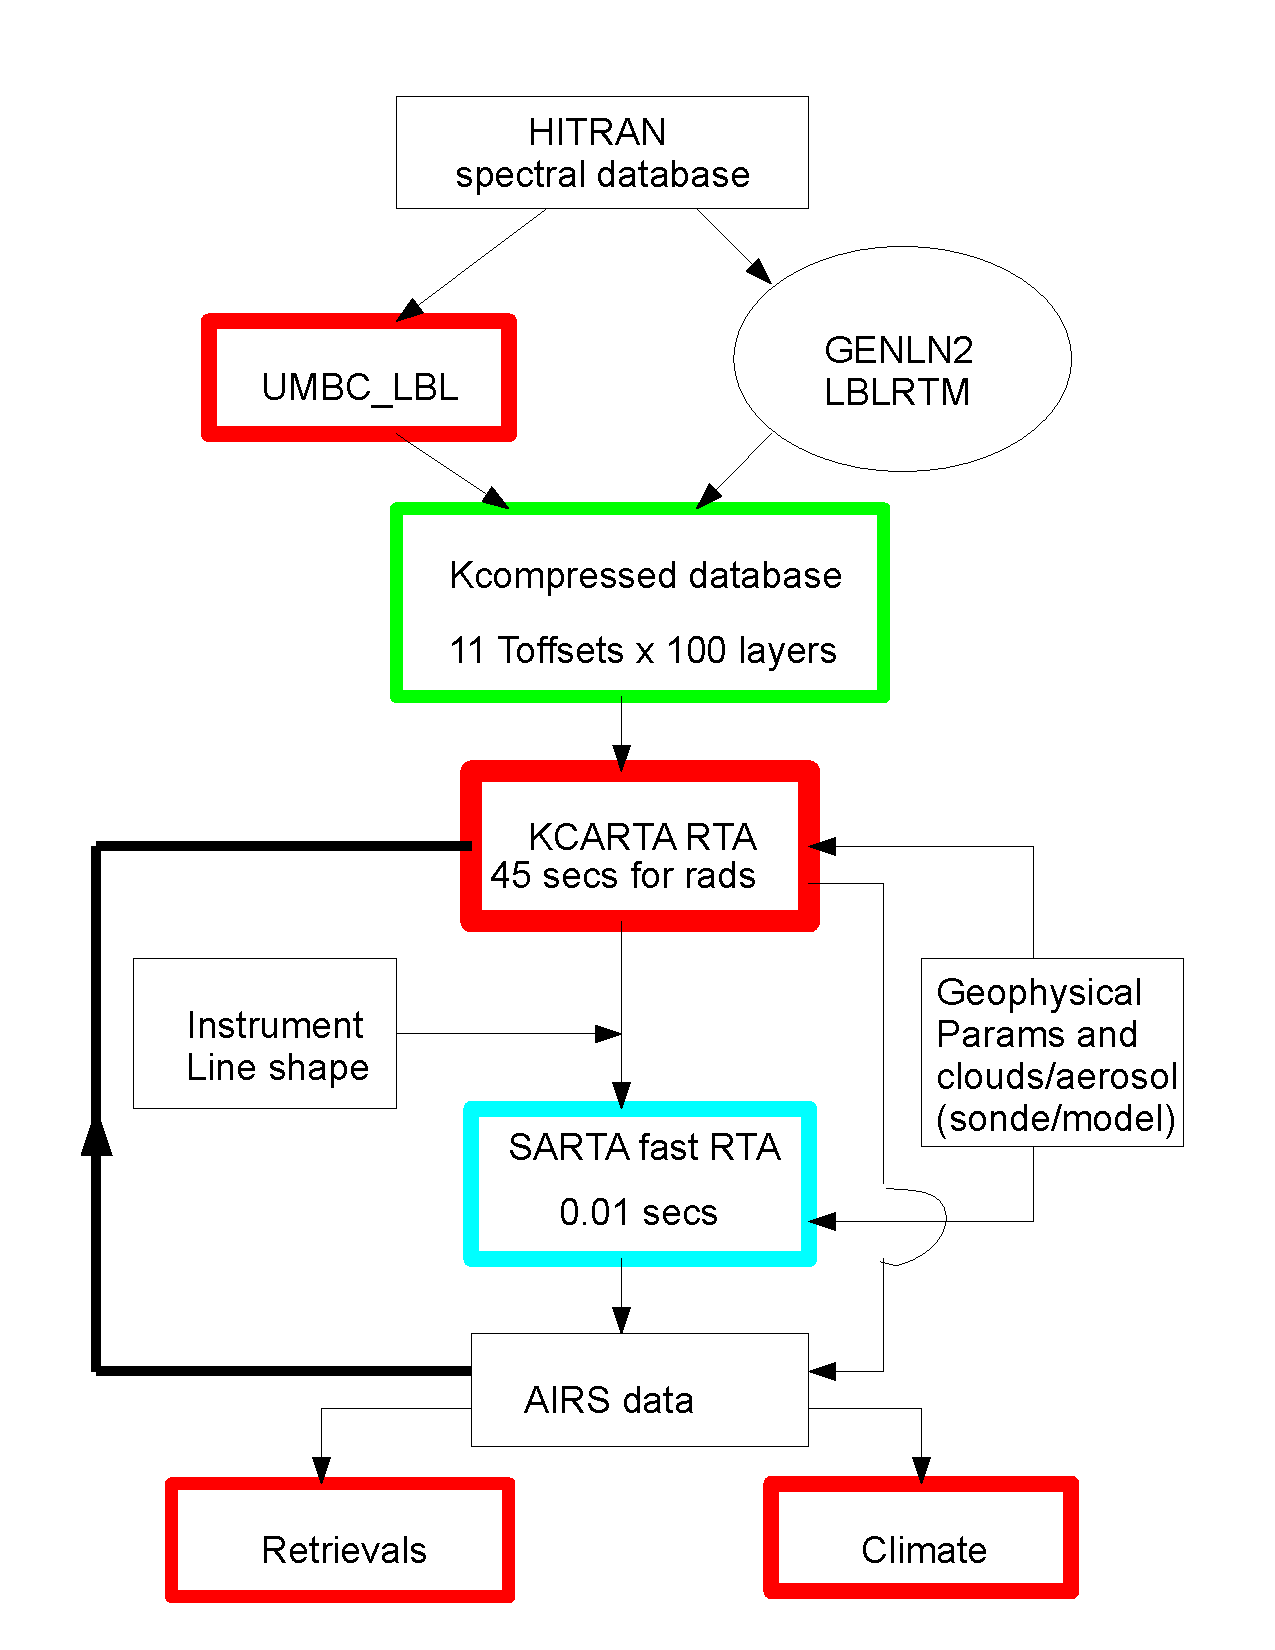
\includegraphics[width=0.5\textwidth]{kcarta_sarta.pdf}
%   \end{center}
% \end{frame}
% ---------------------------------------------------------------------
% ---------------------------------------------------------------------
\section{kCARTA}
% ---------------------------------------------------------------------
% ---------------------------------------------------------------------
\begin{frame}
  \frametitle{KCARTA Details}
  \begin{itemize}
  \item Uses various HITRAN databases and water continuum models
  \item In addition to IR Sounder Spectral region we have 15-605 \wn, 2830-44000 \wn capability
  \item Clear/cloudy sky calculation includes fast analytic jacobians
  \item Background thermal done at each layer/wavenumber point with
    variable diffusivity angle
  \item Fluxes/heating rates can be computed
  \end{itemize}
\end{frame}
% -------------------------------------------------------------------------------------
\begin{frame}
  \frametitle{kCARTA Development: Continual!}
  \vspace{-0.15in} \small\textcolor{blue}{(blue = under development)}

  {\bf \textcolor{maroon}{Have continually updated kCARTA with each HITRAN
      release} } \vspace{-0.1in}

  \begin{small}
    \begin{itemize} \itemsep0.25pt
    \item Past: 1996,2000,2004,2008,2012 .. \textcolor{maroon}{now have
        2016}
    \item Recent addition: GEISA 2015 (European ``HITRAN'')

    \end{itemize}
  \end{small}

  \textcolor{maroon}{\water : }"without basement" plus continuum (MT-CKD
  2.5, 3.2) \vspace{-0.1in}
  \begin{small}
    \begin{itemize} \itemsep0.25pt
    \item \textcolor{blue}{kCARTA has HDO; will break out HDO scaling for
        future SARTAs}
    \end{itemize}
  \end{small}

  \textcolor{maroon}{\cd :} UMBC line mixing based on 1998 data/HITRAN
  \vspace{-0.1in}
  \begin{small}
    \begin{itemize} \itemsep0.25pt
    \item Can use LBLRTM \cd line mixing, v12.4, 12.8, (from Hartmann)
    \item \textcolor{blue}{HITRAN now provides line mixing package from
        Hartmann, HITRAN have just given me new package.}
    \item \textcolor{blue}{non-LTE fitting} : Updated for HITRAN 2016
    \item \textcolor{blue}{4.3 $\mu$m collision induced absorption:
        \cd:\nitrogen, and now \cd:\water Hartmann}
    \end{itemize}
  \end{small}

  \textcolor{maroon}{\methane : } Our LBL code defaults to Voigt lineshape
  \vspace{-0.1in}
  \begin{small}
    \begin{itemize} \itemsep0.25pt
    \item LBLRTM has \methane line mixing, now used in SARTA
    \end{itemize}
  \end{small}

\end{frame}
% -------------------------------------------------------------------------------------
% ---------------------------------------------------------------------
\subsection{Uncertainities}
% ---------------------------------------------------------------------
% ---------------------------------------------------------------------
\begin{frame}
  \frametitle{Comparing \cd line mixing, \methane databases}

  \begin{columns}

    \begin{column}{0.55\columnwidth}
      \begin{block}{\hspace{0.2in}\cd 15$\mu$m}
        \small  I. Gordon (HITRAN) has just given me updated \cd linemixing package\\
        \vspace{0.2in}      
        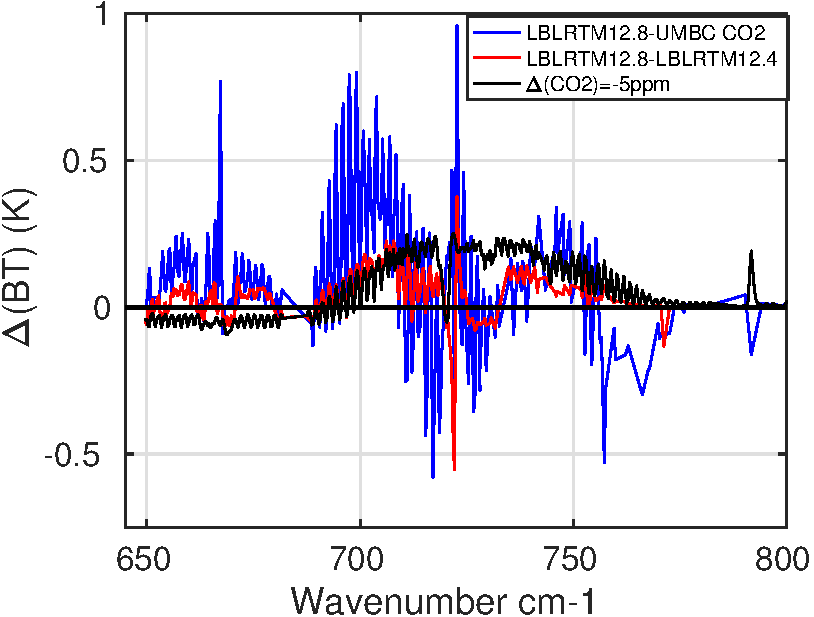
\includegraphics[width=\linewidth]{Figs/FigsHITRAN/co2_intercompare_different_models2.pdf}
      \end{block}
    \end{column}

    \begin{column}{0.55\columnwidth}
      \begin{block}{\methane line mixing}
        \small  LBLRTM has \methane line mixing (H2012), we do not (H2016)\\
        \vspace{0.2in}
        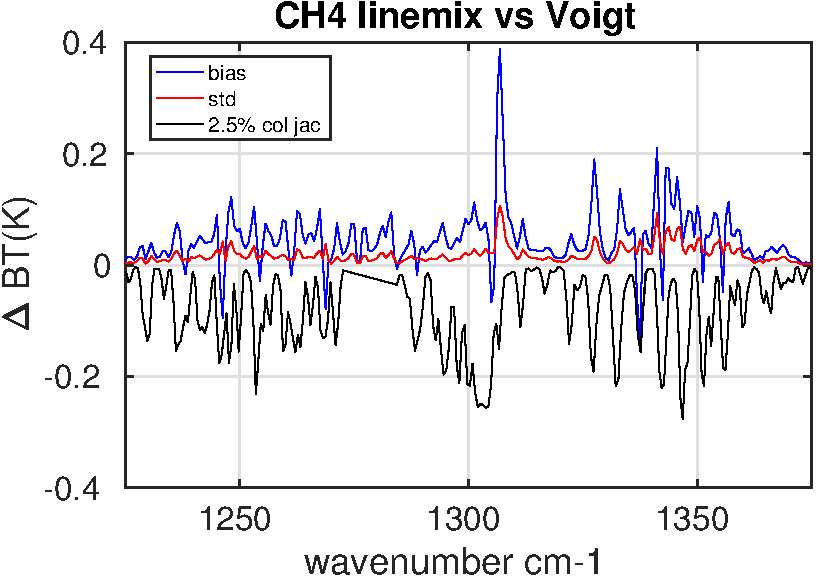
\includegraphics[width=\linewidth]{Figs/FigsH16_G15/ch4linemix3.pdf}
      \end{block}
    \end{column}

  \end{columns}

\end{frame}
% ---------------------------------------------------------------------
\begin{frame}
  \frametitle{Assessing HITRAN 2012 vs HITRAN 2016 vs GEISA 2015}

  \begin{columns}

    \begin{column}{0.55\columnwidth}
      \begin{block}{HITRAN-16 vs HITRAN-12}
        \small   Not all xsec gases that I use are in GEISA (will soon be fixed)\\
        \vspace{0.2in}
        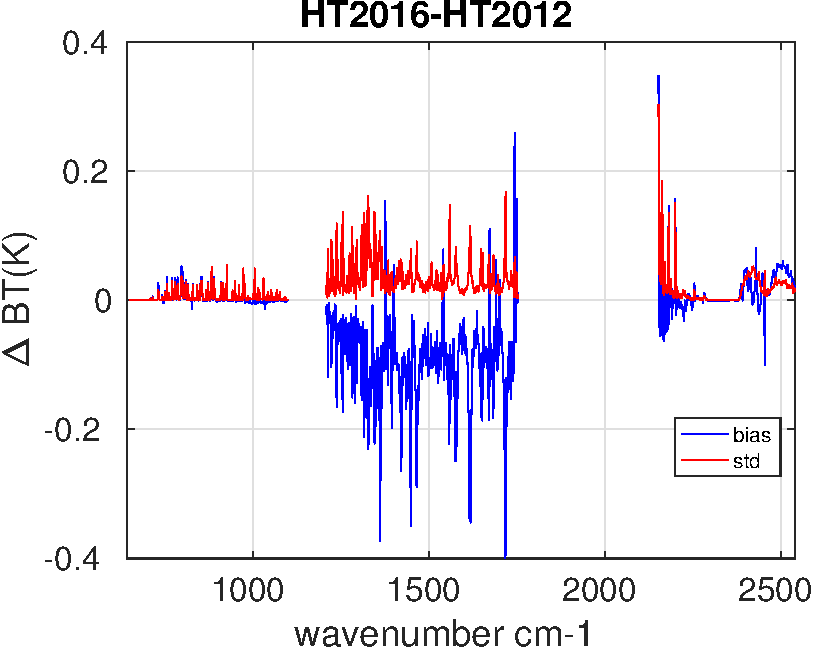
\includegraphics[width=\linewidth]{Figs/FigsH16_G15/h16_h12_v2.pdf}
      \end{block}
    \end{column}

    \begin{column}{0.55\columnwidth}
      \begin{block}{HITRAN-16 vs GEISA-15}
        \small   Not all xsec gases that I use are in GEISA (will soon be fixed)\\
        \vspace{0.2in}
        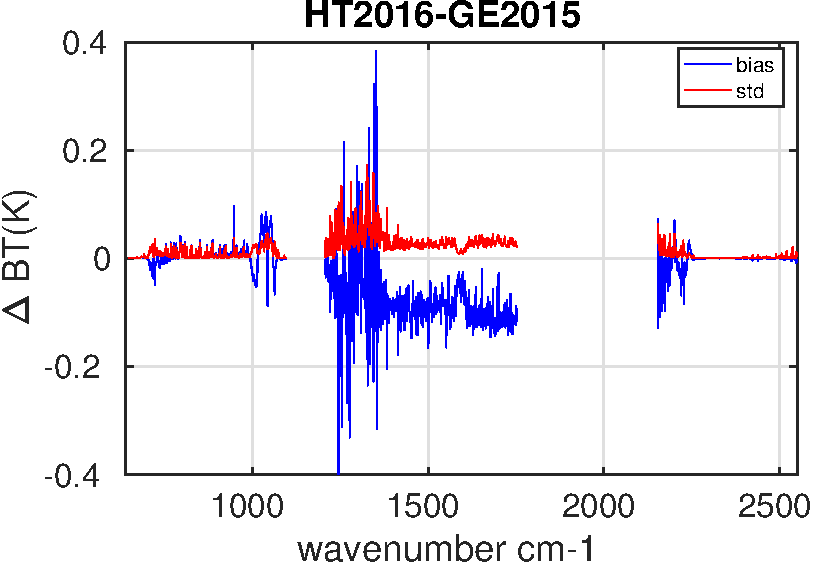
\includegraphics[width=\linewidth]{Figs/FigsH16_G15/h16_g15_v2.pdf}
      \end{block}
    \end{column}

  \end{columns}
  
\end{frame}
% ---------------------------------------------------------------------
% ---------------------------------------------------------------------
\section{SARTA}
% --------------------------------------------------------------------
% ---------------------------------------------------------------------
\begin{frame}\frametitle{Fast Radiative Transfer (SARTA)}
  \begin{itemize}
  \item Validated against kCARTA LBL and statistical analysis of large test
    data sets.
  \item Allows computation of SARTA error covariance matrix (for
    parmeterization errors)
  \item Clear/cloudy RT calcs using eg sonde (clear) or NWP model fields
    (cloudy)
  \item Many minor gases included
  \item Emissivity and reflectance
    \begin{itemize}
    \item Ocean emissivity by Masuda (wind speed dependance)
    \item Land emissivity by U. Wisc or NASA Langley
    \item \textcolor{blue}{Daytime over ocean bi-directional reflectance
        (Nalli et. al.)}
    \end{itemize}
  \end{itemize}
\end{frame}
% --------------------------------------------------------------------
\begin{frame}
  \frametitle{Latest CrIS FSR SARTA}
  Already delivered
  
  \begin{itemize}
  \item HITRAN 2012 (molecular and xsec gases)
  \item MT-CKD 2.5
  \item LBLRTM v12.4 : \cd and \methane line mixing
  \end{itemize}

  Future plans (roughly ordered by increasing complexity)
  \begin{itemize}
  \item \amm + MT-CKD3.2 + HITRAN2016
  \item HDO (column mult wrt \water is easy; 100 layer more involved)
  \item Updated \cd line mixing (depends on kCARTA tests)
  \item 4.3 um bandhead \cd/\water and \cd/\nitrogen CIA (depends on kCARTA
    tests)
  \item Move from linear regression to Gaussian Kernel Regression?
    \begin{itemize}
    \item LLS is straighforward but can be inaccurate ``outside training''
    \item GKR is more accurate esp ``outside training'' regime; very
      promising but much more complex
    \end{itemize}
  \item \textcolor{blue}{New parameterization with simplified algorithm
      (longer term)}
  \end{itemize}
  
\end{frame}
% ---------------------------------------------------------------------
\begin{frame}
  \frametitle{New Spectroscopy For LBL (J.M. Hartmann/H. Tran)}
  \vspace{-0.1in} Recent work by J.M. Hartmann/H. Tran and others (HITRAN
  2018 Conference) indicate that N$_2$-\water and \cd-\water collisions are
  important for the 4.3 $\mu$m band head!  Significant effort to
  incorporate into LBL and separate from existing \water continuum.

  \vspace{-0.1in}
  \begin{columns}

    \begin{column}{0.55\columnwidth}
      \begin{block}{Lab Spectra}
        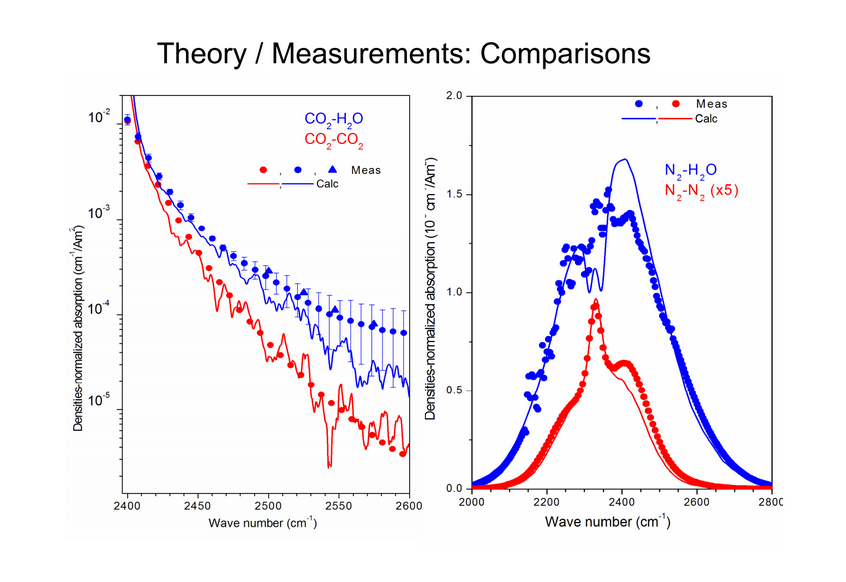
\includegraphics[width=\linewidth]{HartmannSlide1.png}
      \end{block}
    \end{column}

    \begin{column}{0.55\columnwidth}
      \begin{block}{IASI Biases}
        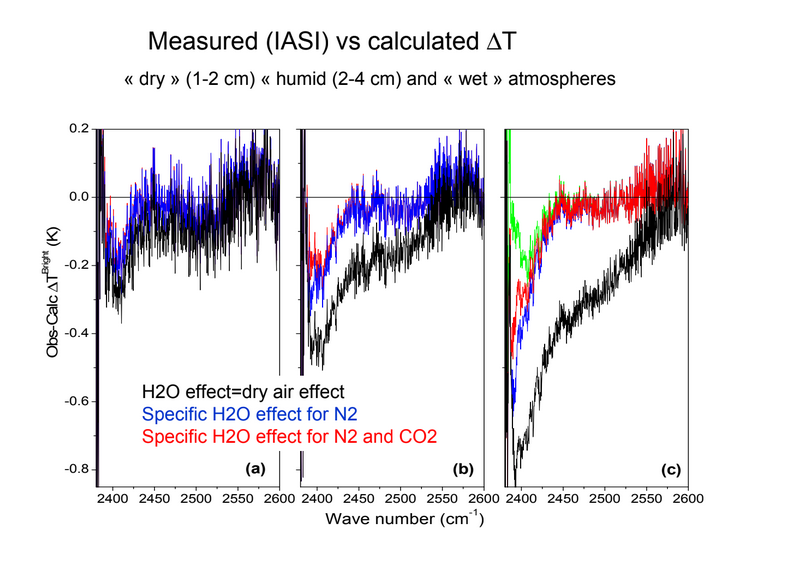
\includegraphics[width=\linewidth]{HartmannSlide2.png}
      \end{block}
    \end{column}

  \end{columns}

\end{frame}
% --------------------------------------------------------------------
\begin{frame}\frametitle{SARTA vs kCARTA comparison (49 regr profiles)}
  \centering
  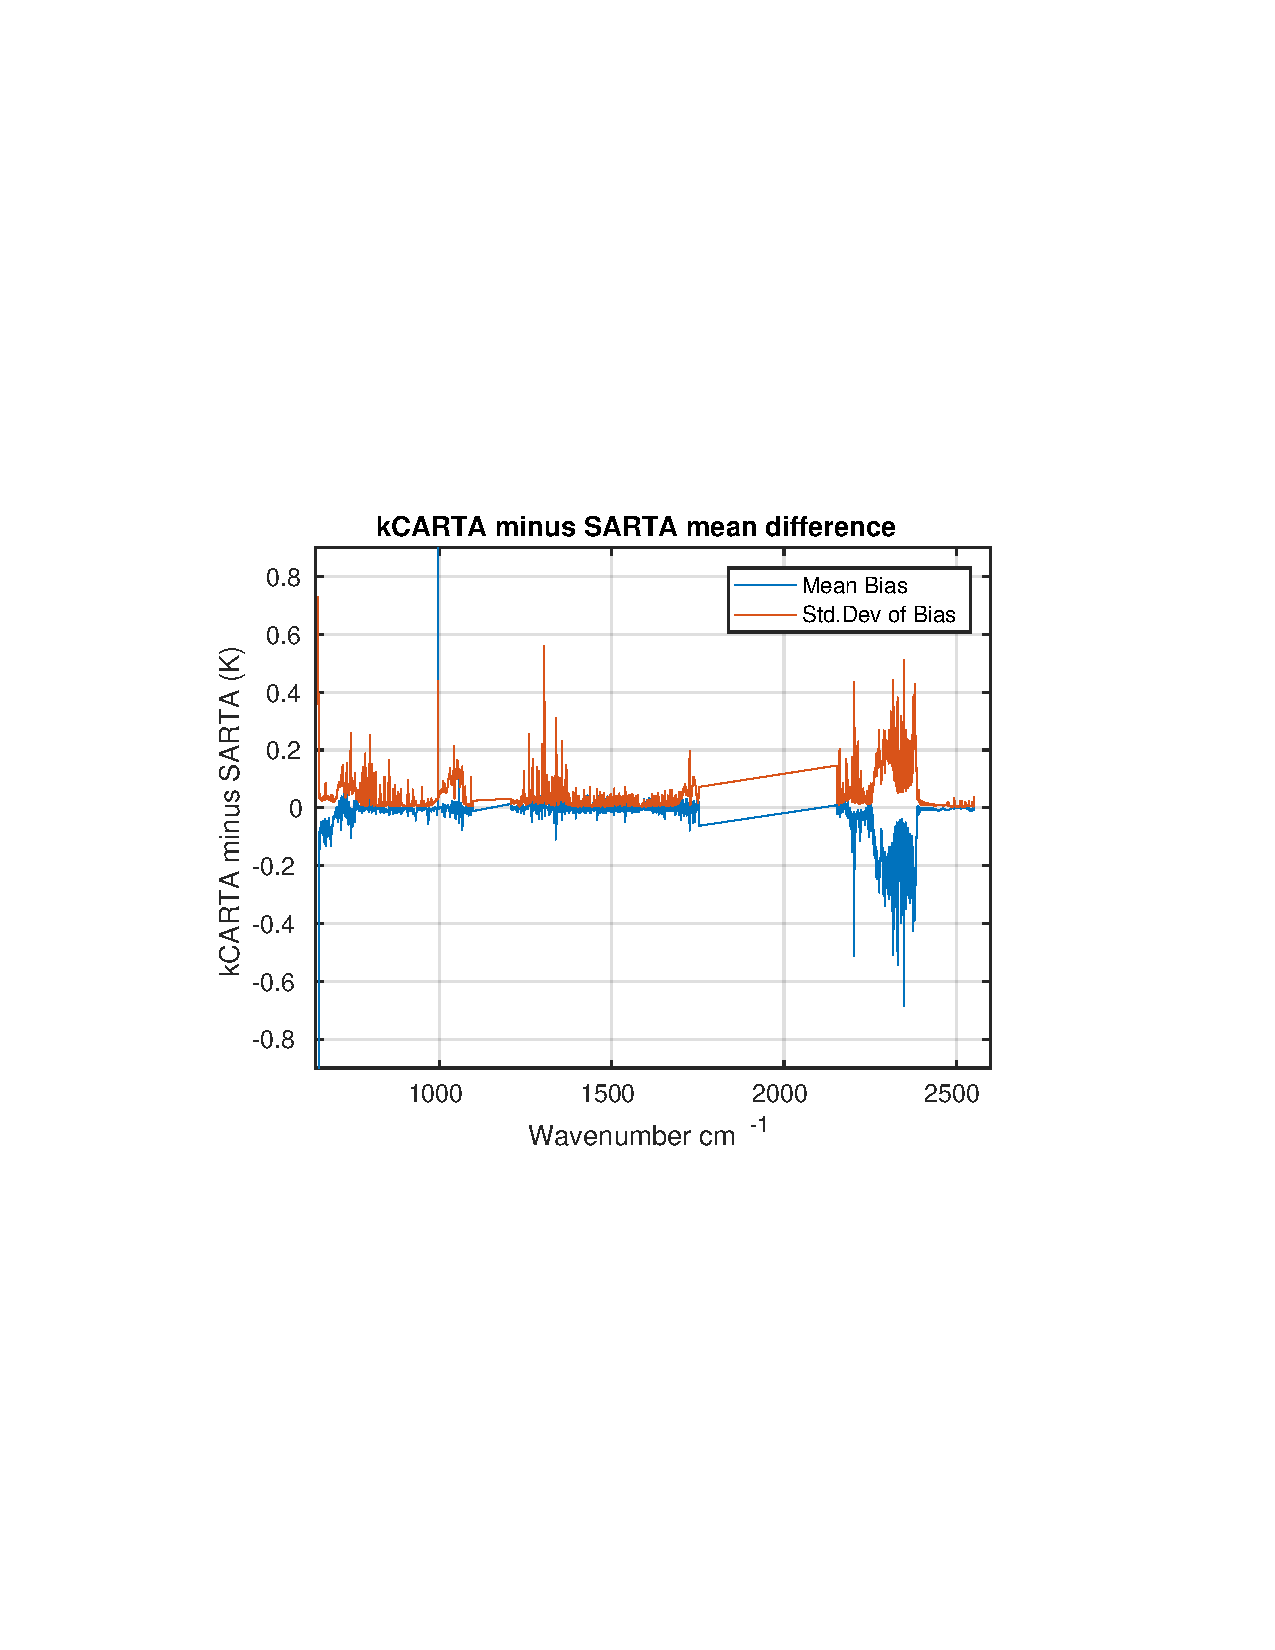
\includegraphics[width=0.95\linewidth]{./r49_kcarta_sarta_bias_std_spectrum.pdf}
\end{frame}
% --------------------------------------------------------------------
\begin{frame}\frametitle{\amm : SARTA vs KCARTA}
  \centering
  % 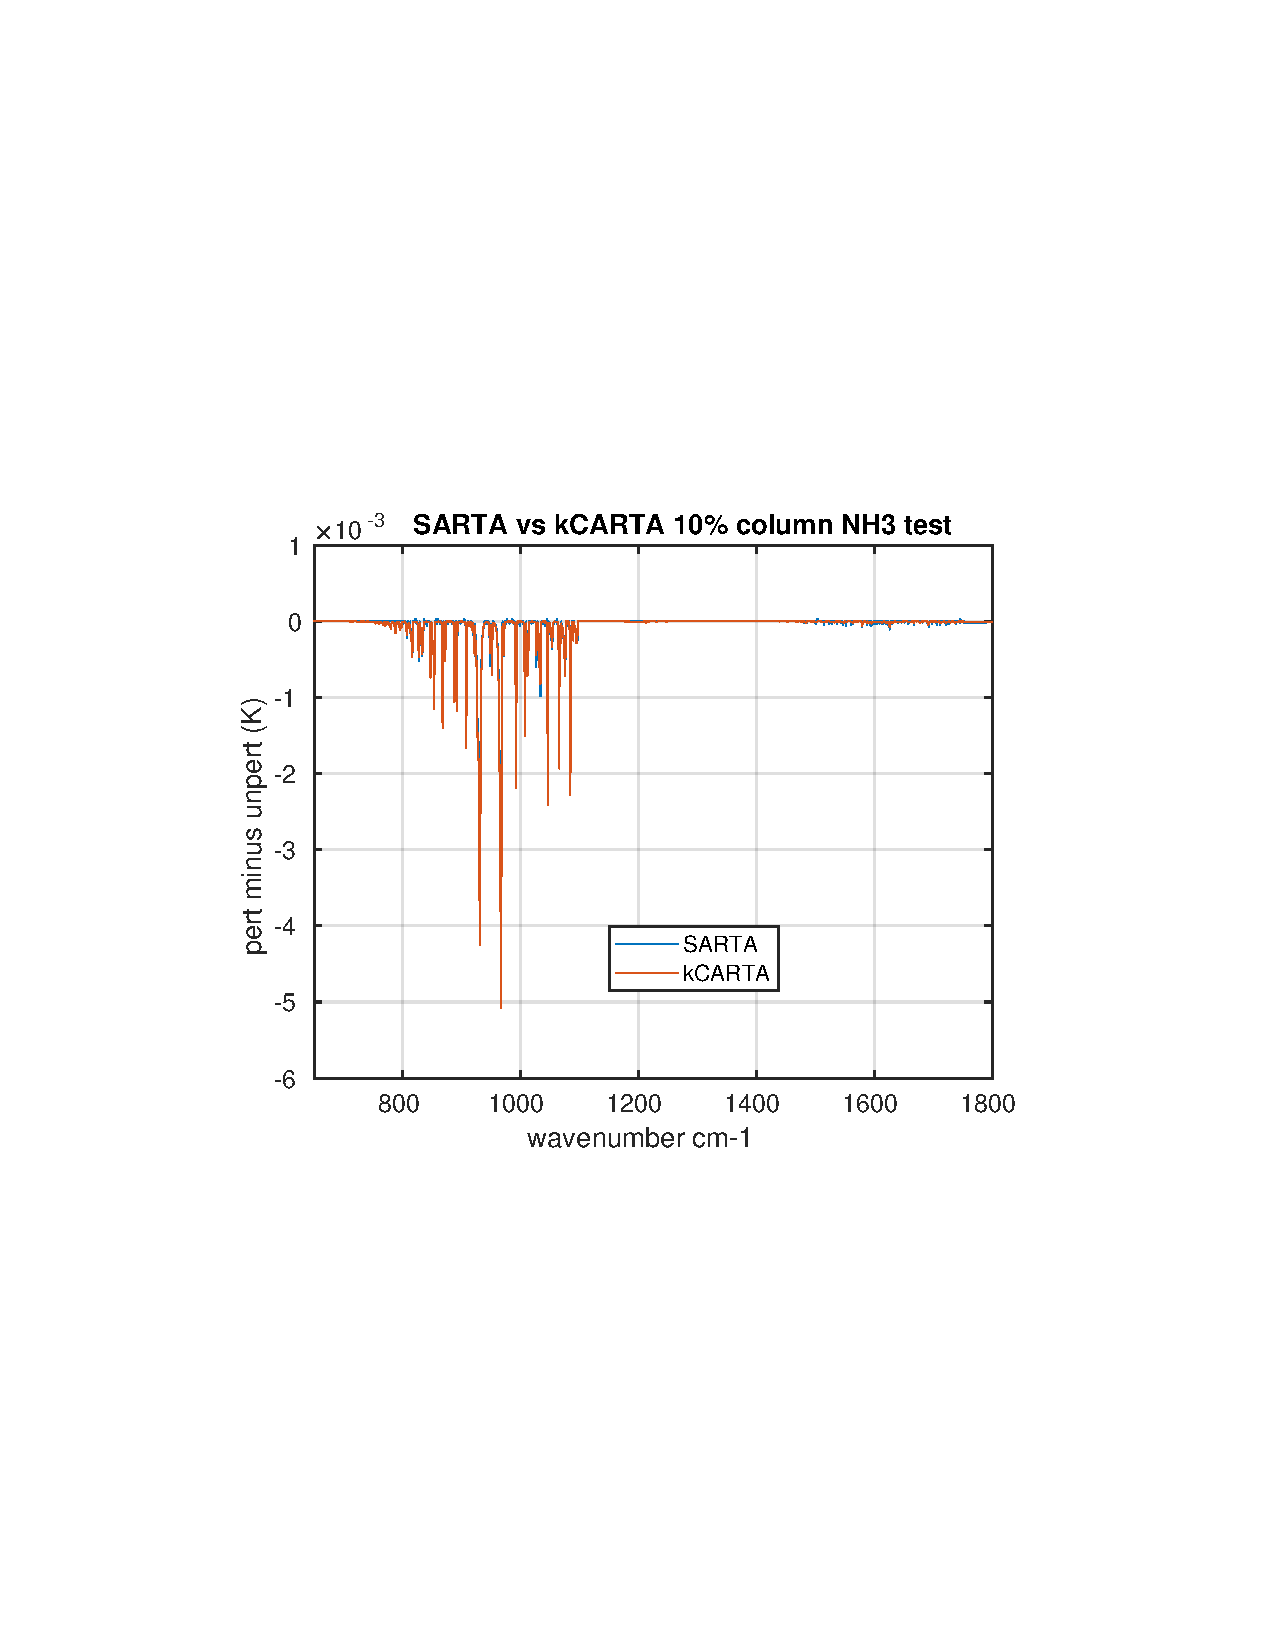
\includegraphics[width=0.9\linewidth]{./sarta_kcarta_nh3_perturb_unitemis.pdf}
  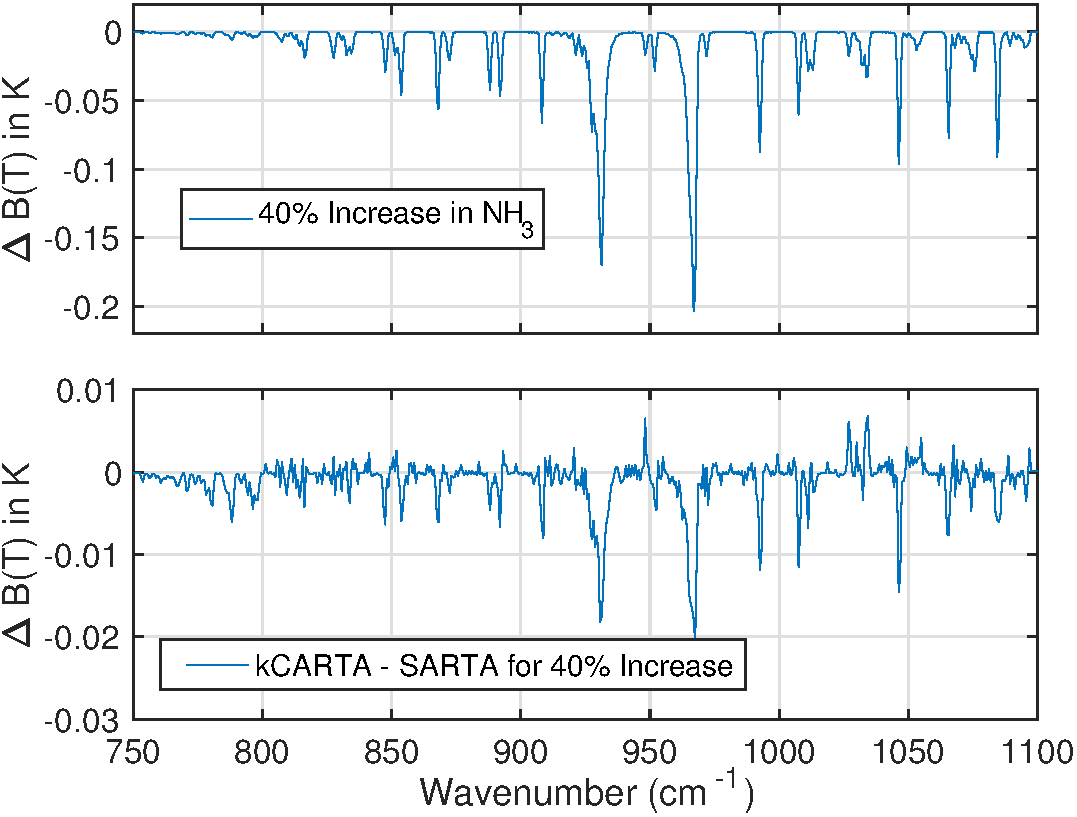
\includegraphics[width=0.9\linewidth]{lls_nh3.pdf} \newline Small, mostly
  systematic errors (4\% error for 40\% variation in \amm).
\end{frame}
% --------------------------------------------------------------------
\begin{frame}[shrink=20]
  \frametitle{Existing and Upcoming Versions}

  \begin{block}{AIRS Level 2 Processing}
    \begin{itemize}
    \item HITRAN 2008
    \item Dual frequency set, L2 algorithm interpolates to the correct frequency  dynamically 
     \end{itemize}
  \end{block}
  \begin{block}{CrIS FSR}
    \begin{itemize}
    \item HITRAN 2012
    \item Improved reflected thermal.
     \end{itemize}
  \end{block}
  \begin{block}{NASA Continuity Processing}
    \begin{itemize}
    \item If use present RTAs, will be mixing HITRAN 2008 and HITRAN 2012, etc
    \item We have built a prototype AIRS L1c HITRAN 2016 code
      \begin{itemize}
      \item Validation not yet complete.
      \item Doesn't have latest Hartmann spectroscopy shown above
      \end{itemize}
    \item Suggestion for first AIRS + CrIS Level 2 data set
      \begin{itemize}
      \item We complete a prototype AIRS L1c RTA (HITRAN 2016 + maybe Hartmann)
      \item We update CrIS RTA (to HITRAN 2016 + maybe Hartmann)
      \item This takes away time from improving the parameterization, but maybe worth it.
      \end{itemize}
  
      

    \end{itemize}
  \end{block}
  
  
\end{frame}
% --------------------------------------------------------------------
\begin{frame}
  \frametitle{Conclusions}
  \begin{itemize}
  \item We have been concentrating on spectroscopy and line-by-line
    improvements
  \item \cd lineshape changes are particulary important because they are
    \emph{not} static but depend on the \water burden.
  \item We have shown (Lindeberg) that HITRAN 2016 \water is slightly
    better than HITRAN 2012 (not discussed)
  \item Improvement to kCARTA can be migrated to SARTA quickly (with
    current parameterization)
  \item \textcolor{maroon}{Larrabee and Chris working on SRFs for AIRS L1c}
  \item \textcolor{maroon}{Next delivery : HITRAN16, updated \cd line-mix,\amm, HDO}
  \end{itemize}
\end{frame}
% --------------------------------------------------------------------
% --------------------------------------------------------------------
\end{document}
% --------------------------------------------------------------------
% --------------------------------------------------------------------

%%% Local Variables:
%%% mode: latex
%%% TeX-master: t
%%% End:
